\subsection{}

\begin{definition}
    Market Economy is an economy where resources are allocated through the decentralized decisions of many firms and households as they interact in markets for goods and services.
    The economy is characterized by being self-organizing and efficient.
    We assume that the agents of the market are self-interested and incentivized.
\end{definition}

The Three agents are individuals, firms and government and are all interested in maximizing something.
Individuals maximize utility (happiness), firms maximize profit and government maximizes social welfare (in an ideal world).

\begin{definition}
    Incentives are rewards or penalties that motivate behaviour.
\end{definition}

\begin{definition}
    Free Trade is the policy of not discriminating against imports from other countries and relying on the market to allocate resources.
\end{definition}

\begin{definition}
    Protectionism is the policy of protecting domestic industries against foreign competition by imposing tariffs, quotas and other trade barriers.
\end{definition}

\begin{example}
    Let us focus on two agents: individuals and firms and three markets: goods and services, financial and factor.
    \begin{figure}[h!]
        \centering
        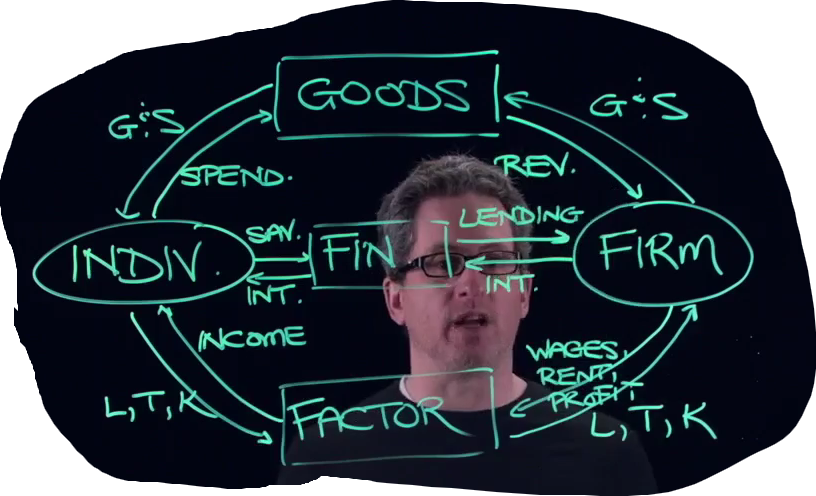
\includegraphics[width=0.5\textwidth]{CircularFlowOfIncomeAndExpenditure.png}
        \caption{Circular Flow of Income and Expenditure}
    \end{figure}
    Firms provide goods and services to the goods and services market and expect revenue.
    The factor market provides firms with resources (T, L and K) and expect wages, rent and profit.
    Individuals receive income (wages, rent and profit) from the factor market and provide resources (T, L and K).
    Individuals spend their income on goods and services in the goods and services market.
    Individuals save their income in the financial market and expect interest.
    Firms lend from the financial market and the market expects interest.

\end{example}
